\section{raytrace.2d and raytrace.3d - Geometric Acoustics}

Geometrical acoustics is not heavily supported because of the availability of advanced geometrical acoustics packages elsewhere. See, for example, the GeoAc package available from the Los Alamos National Laboratory at https://github.com/philblom/GeoAc/archive/master.zip. Included here are {\bf raytrace.2d} and {\bf raytrace.3d}. These are range-independent geometric infrasound propagation algorithms for computing raypaths and signal transmission loss relative to 1 km in the Effective Sound Speed Approximation. The algorithms return a 2-D (r and z) or 3-D (x, y, and z) trace of the raypath calculated for a given elevation and azimuth.  The 2-D calculation uses the effective sound speed approximation for its computation, while the 3-D calculation uses a moving-medium formulation.

\subsection{Mathematical Background: 2-D}
\label{sec: raytrace.2d math}

The mathematical structure of the 2-D geometrical acoustics module is fully described in \cite{blom_jasa}.  Let $r$ be the range along the propagation path, $z$ be the altitude, $\theta$ be the takeoff angle, and $c_{eff}(z)$ be the effective sound speed in the propagation direction at $z$.  Define the following auxiliary quantities:

\begin{equation}
\mathcal{R}\equiv\frac{\partial r}{\partial\theta},
\mathcal{Z}\equiv\frac{\partial z}{\partial\theta},
\eta\equiv\frac{\partial\zeta}{\partial\theta}
\end{equation}

The 2-D geometric acoustics calculation is then performed by using a 4th-order Runge-Kutta method to solve the following system of 6 equations:

\begin{equation}
\frac{dr}{ds}=\frac{c_{eff}(z)}{c_{eff}(0)}\cos\theta
\label{eq: 2d-drds}
\end{equation}
\begin{equation}
\frac{dz}{ds}=c_{eff}(z)\zeta(s,\theta)
\label{eq: 2d-dzds}
\end{equation}
\begin{equation}
\frac{d\zeta}{ds}=-\frac{c_{eff}'(z)}{c_{eff}^2(z)}
\label{eq: 2d-dzetads}
\end{equation}
\begin{equation}
\frac{d\mathcal{R}}{ds}=\frac{c_{eff}'(z)}{c_{eff}(0)} \mathcal{Z}(s,\theta)\cos\theta - \frac{c_{eff}(z)}{c_{eff}(0)}\sin\theta
\label{eq: 2d-dRds}
\end{equation}
\begin{equation}
\frac{d\mathcal{Z}}{ds}=c_{eff}'(z)\mathcal{Z}(s,\theta)\zeta(s,\theta) + c_{eff}(z)\eta(s,\theta)
\label{eq: 2d-dZds}
\end{equation}
\begin{equation}
\frac{d\eta}{ds}=\left[2\left(\frac{c_{eff}'(z)}{c_{eff}(z)}\right)^2 - \frac{c_{eff}''(z)}{c_{eff}(z)}\right]\frac{\mathcal{Z}(s,\theta)}{c_{eff}(z)}
\label{eq: 2d-detads}
\end{equation}


\subsection{Running raytrace.2d}
\label{sec: raytrace.2d running}

Making sure that the executable for {\bf raytrace.2d} is in the system's path, it can be run by entering 
\begin{verbatim} 
    raytrace.2d [--option1 val1] [--option2 val2] [...] [--flag1] [...] 
\end{verbatim}
on a command line. Generally, options are followed by values, either numbers, strings or filenames. Flags are not. Entering \verb"raytrace.2d" without any options or flags sends the following help page to the screen: 

\begin{verbatim}
Usage: 

The options below can be specified in a colon-separated file "raytrace.2d.options" or at
the command line.  Command-line options override file options.
 --help -h                Print this message and exit

To use an arbitrary 1-D atmospheric profile in ASCII format (space or comma-separated) 
the following options apply:
REQUIRED (no default values):
 --atmosfile  <filename>  Uses an ASCII atmosphere file
 --atmosfileorder         The order of the (z,t,u,v,w,p,d) fields in the ASCII file 
                          (Ex: 'ztuvpd')
 --elev                   Value in range (-90,90)
 --azimuth                Value in range [0,360), clockwise from north
 --maxraylength           Maximum ray length to calculate (km) [none]
OPTIONAL [defaults]:
 --skiplines              Lines at the beginning of the ASCII file to skip [0]
 --maxelev                Maximum elevation angle to calculate [--elev value]
 --delev                  Elevation angle step [1]
 --maxazimuth             Maximum azimuth to calculate [--azimuth value]
 --dazimuth               Azimuth angle step [1]
 --sourceheight           Height at which to begin raytrace [ground level]
 --maxheight              Height at which to cut off calculation [150 km]
 --maxrange               Maximum distance from origin to calculate (km) [no maximum]
 --stepsize               Ray length step size for computation, km [0.01]
 --skips                  Maximum number of skips to allow.  Use 0 for no limits.  [0]
 --wind_units             Specify 'kmpersec' if the winds are given in km/s [mpersec]
FLAGS (no value required):
 --partial                Report the final, incomplete raypath as well as the complete 
                          bounces.

Examples (run from 'samples' directory):
../bin/raytrace.2d --azimuth 90 --elev 1 --delev 1 --maxelev 45 --skips 1 \
--atmosfile NCPA_canonical_profile_zuvwtdp.dat --atmosfileorder zuvwtdp \
--maxraylength 800 --maxheight 140
cat raypath_az090* > raypaths.2d.dat
rm raypath_az090*
\end{verbatim}

To use {\bf raytrace.2d} an ascii file containing the atmospheric specifications must be loaded using the option \verb+--atmosfile+ followed by the filename. The order of the columns in the specification file needs to be specified using \verb+--atmosfileorder+ followed by a string indicating the order; eg. zuvwtdp if the columns orders are altitude, zonal wind, meridional wind, vertical wind, temperature, density and pressure. Units are as indicated. The option \verb+--skiplines+, followed by a non-negative integer, is generally used to skip any header lines that might be in the file.

The output is a set of space-delimited ASCII file with columns for r (range, km), z (height, km), and A (amplitude relative to 1km).  A shell-style commented header contains summary information about the azimuth and elevation angles used to generate the file, as well as calculated values for turning height, final range, travel time and celerity.  Each file is named as "raypath\_az[azimuth]\_elev[elevation].txt".

\subsection{Running raytrace.2d: examples}
\label{sec: raytrace.2d examples}

The \textbf{raytrace.2d} help page ends with one example command, a simple example illustrating the primary input modes for raytrace.2d. It is assumed that the user runs it in the \verb+samples+ directory. Note that if the \textbf{ncpaprop} \verb+bin+ directory is in the system's path one may enter \verb+raytrace.2d+ rather than \verb+../bin/raytrace.2d+. The command line entry for the example is 
\begin{verbatim} 
    ../bin/raytrace.2d --azimuth 90 --elev 1 --delev 1 --maxelev 45 --skips 1 \
                       --atmosfile NCPA_canonical_profile_zuvwtdp.dat \
                       --atmosfileorder zuvwtdp --maxraylength 800 --maxheight 140
\end{verbatim}


Ground-to-ground propagation in the NCPA toy atmosphere (see Figure 1) at 90 degrees azimuth (from North), eastward propagation is modelled Propagation parameters are given in \verb"raytrace.2d.options" or, as here, can be specified on the command line. The calculation is stopped if the ray exceeds 140 km in altitude or hits the ground (only 1 skip is requested), or if the total raypath length exceeds 800 km. The atmospheric profiles are specified in a column-based text file \verb"NCPA_canonical_profile_zuvwtdp.dat". The column order is specified with option \verb"--atmosfileorder". In the above example the profile file has 7 columns in the following order \verb"zuvwtdp" (refer to section~\ref{sec: AtmoSpecs}  for an explanation of atmospheric specifications).  The atmospheric file used should always extend past the maximum height used for the calculation, or the program will crash.

The output from the example command is shown in Figure \ref{fig:RT2D}.\newline 

\begin{figure}
\begin{center}
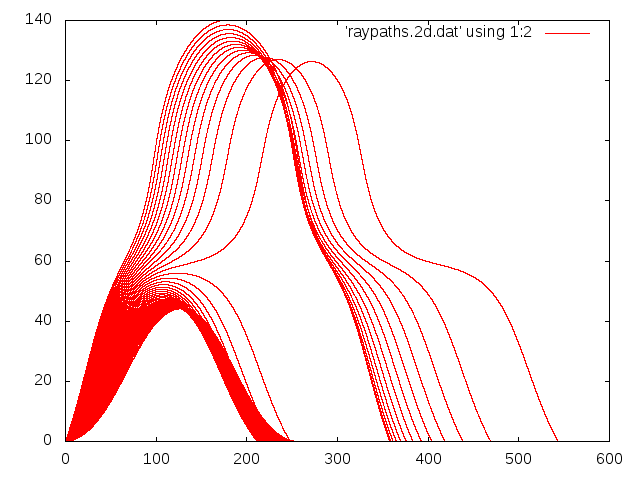
\includegraphics[scale=0.45]{figs/raytrace2d}
\end{center}
\caption{2D ray trace output for the example commands provided.}
\label{fig:RT2D}
\end{figure}


\subsection{Mathematical Background: 3-D}
\label{sec: raytrace.3d math}

The mathematical structure of the 3-D geometrical acoustics module is fully described in \cite{blom_dissertation}.  Let $\vec{x}$ be the displacement vector and $\nu$ be the Eikonal equation for propagation in three dimensions, $\vec{c_p}$ be the propagation velocity, $c$ be the thermodynamic sound speed, and $\vec{v_0}$ be the wind.  The 3-D module uses a 4th-order Runge-Kutta method to solve the coupled equations

\begin{equation}
\frac{\partial\vec{x}}{\partial s}=\frac{\vec{c_p}}{c_p}
\label{eq: 3d-delxdels}
\end{equation}
\begin{equation}
\frac{\partial\nu_j}{\partial s}=-\frac{1}{c_p} \left[\nu\frac{\partial c}{\partial x_j} + \vec{\nu}\cdot\frac{\partial\vec{v_0}}{\partial x_j}\right]
\label{eq: 3d-delnudels}
\end{equation}

Twelve other equations are also solved, which represent

\begin{equation}
\frac{\partial}{\partial s}\left(\frac{\partial\vec{r}}{\partial\theta},\frac{\partial\vec{\nu}}{\partial\theta},\frac{\partial\vec{r}}{\partial\phi},\frac{\partial\vec{\nu}}{\partial\phi}\right)
\label{eq: 3d-angular}
\end{equation}

These equations are voluminous in their expanded forms and are not reproduced here.

\subsection{Running raytrace.3d}
\label{sec: raytrace.3d running}

Making sure that the executable for {\bf raytrace.3d} is in the system's path, it can be run by entering 
\begin{verbatim} 
    raytrace.3d [--option1 val1] [--option2 val2] [...] [--flag1] [...] 
\end{verbatim}
on a command line. Generally, options are followed by values, either numbers, strings or filenames. Flags are not. Entering \verb"raytrace.3d" without any options or flags sends the following help page to the screen: 

\begin{verbatim}
Usage: 

The options below can be specified in a colon-separated file "raytrace.3d.options" or at 
the command line.  Command-line options override file options.
 --help -h                Print this message and exit

To use an arbitrary 1-D atmospheric profile in ASCII format (space or comma-separated) 
the following options apply:
REQUIRED (no default values):
 --atmosfile  <filename>  Uses an ASCII atmosphere file
 --atmosfileorder         The order of the (z,t,u,v,w,p,d) fields in the ASCII file 
                          (Ex: 'ztuvpd')
 --elev                   Value in range (-90,90)
 --azimuth                Value in range [0,360), clockwise from north
 --maxraylength           Maximum ray length to calculate (km) [none]
OPTIONAL [defaults]:
 --skiplines              Lines at the beginning of the ASCII file to skip [0]
 --maxelev                Maximum elevation angle to calculate [--elev value]
 --delev                  Elevation angle step [1]
 --maxazimuth             Maximum azimuth to calculate [--azimuth value]
 --dazimuth               Azimuth angle step [1]
 --sourceheight           Height at which to begin raytrace [ground level]
 --maxheight              Height at which to cut off calculation [150 km]
 --maxrange               Maximum distance from origin to calculate (km) [no maximum]
 --stepsize               Ray length step size for computation, km [0.01]
 --skips                  Maximum number of skips to allow.  Enter 0 for no maximum. [0]
 --wind_units             Specify 'kmpersec' if the winds are given in km/s [mpersec]
 FLAGS (no values required):
 --partial                Report the final, incomplete raypath as well as the complete 
                          bounces.

Examples (run from 'samples' directory):
../bin/raytrace.3d --azimuth 90 --elev 1 --delev 1 --maxelev 45 --skips 1 \
--atmosfile NCPA_canonical_profile_zuvwtdp.dat --atmosfileorder zuvwtdp \
--maxraylength 800 --maxheight 140 --skiplines 1
cat raypath_az090* > raypaths.3d.dat
rm raypath_az090*
\end{verbatim}

To use {\bf raytrace.3d} an ascii file containing the atmospheric specifications must be loaded using the option \verb+--atmosfile+ followed by the filename. The order of the columns in the specification file needs to be specified using \verb+--atmosfileorder+ followed by a string indicating the order; eg. zuvwtdp if the columns orders are altitude, zonal wind, meridional wind, vertical wind, temperature, density and pressure. Units are as indicated. The option \verb+--skiplines+, followed by a non-negative integer, is generally used to skip any header lines that might be in the file.

The output is a set of space-delimited ASCII file with columns for x (km), y (km), z (km), A (relative amplitude), and J (Jacobian).  A shell-style commented header contains summary information about the azimuth and elevation angles used to generate the file, as well as calculated values for turning height, final range, travel time and celerity.  Each file is named as "raypath\_az[azimuth]\_elev[elevation].txt".  

\subsection{Running raytrace.3d: examples}
\label{sec: raytrace.3d examples}

The \textbf{raytrace.3d} help page ends with one example command, a simple example illustrating the primary input modes for raytrace.3d. It is assumed that the user runs it in the \verb+samples+ directory. Note that if the \textbf{ncpaprop} \verb+bin+ directory is in the system's path one may enter \verb+raytrace.3d+ rather than \verb+../bin/raytrace.3d+. The command line entry for the example is 
\begin{verbatim} 
    ../bin/raytrace.3d --azimuth 90 --elev 1 --delev 1 --maxelev 45 --skips 1 \
                       --atmosfile NCPA_canonical_profile_zuvwtdp.dat \
                       --atmosfileorder zuvwtdp --maxraylength 800 --maxheight 140
\end{verbatim}


Ground-to-ground propagation in the NCPA toy atmosphere (see Figure 1) at 90 degrees azimuth (from North), eastward propagation is modelled Propagation parameters are given in \verb"raytrace.3d.options" or, as here, can be specified on the command line. The calculation is stopped if the ray exceeds 140 km in altitude or hits the ground (only 1 skip is requested), or if the total raypath length exceeds 800 km. The atmospheric profiles are specified in a column-based text file \verb"NCPA_canonical_profile_zuvwtdp.dat". The column order is specified with option \verb"--atmosfileorder". In the above example the profile file has 7 columns in the following order \verb"zuvwtdp" (refer to section~\ref{sec: AtmoSpecs}  for an explanation of atmospheric specifications).  The atmospheric file used should always extend past the maximum height used for the calculation, or the program will crash.

The output from the example command is shown in Figure \ref{fig:RT3D}. Column 1 ($x$) of the output file is used as the independent variable rather than the magnitude of the x-y vector for the sake of simplicity, since propagation is almost due eastward.\newline

\begin{figure}
\begin{center}
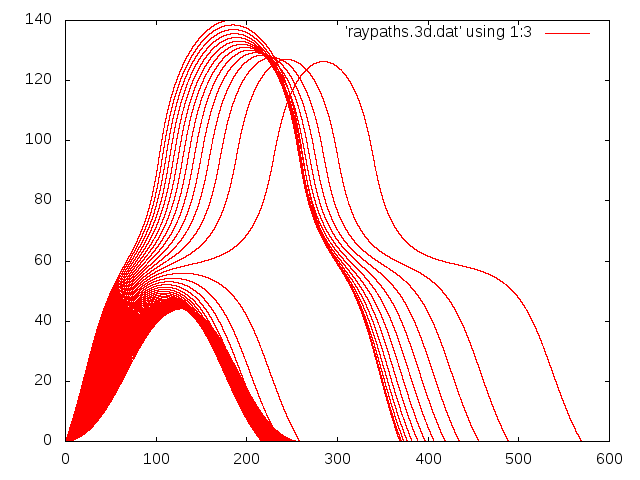
\includegraphics[scale=0.45]{figs/raytrace3d}
\end{center}
\caption{3D ray trace output for the example command provided.}
\label{fig:RT3D}
\end{figure}
 
